\documentclass{beamer}
\usetheme{metropolis}

\usepackage[utf8]{inputenc}
\usepackage[portuguese]{babel}

\usepackage{color}
\usepackage{dirtytalk}
\usepackage{graphicx}
\usepackage{minted}
\usepackage{menukeys}
\usepackage{tabularx}

\graphicspath{{img/}}

\title{Minicurso de Java}
\subtitle{Introdução a Java}
\author{João Paulo Taylor Ienczak Zanette}

\newcommand{\icon}[1]{\raisebox{-.2\height}{\includegraphics[keepaspectratio,width=1em]{#1}}}

\begin{document}

\maketitle

\section{O que é programação?}

\section{Introdução a Java}
\subsection{Sobre a linguagem}

\begin{frame}{Princípios}
    \begin{enumerate}
        \item Deve ser "simples, orientada a objetos, e familiar";
        \item Deve ser "robusta e segura";
        \item Deve ser "de arquitetura neutra e portátil";
        \item Deve executar com "alta performance";
        \item Deve ser "interpretada, dinâmica e com suporte a threads ";
    \end{enumerate}
\end{frame}


\begin{frame}{Características gerais da linguagem}

    \begin{description}
        \item[Multiplataforma:] O mesmo código pode rodar em mais de uma plataforma
            sem a necessidade de recompilar;
        \item[Biblioteca padrão extensa:] Oferece diversos recursos já na
            biblioteca padrão, desde interfaces gráficas até manipulação de
            áudio/vídeo;
        \item[Alocação não-determinística:] Recursos alocados não são liberados
            explicitamente pelo programador, isso é feito por um
            \emph{Garbage-Collector};
        \item[Suporte a JIT:] Alguns trechos de código são otimizados em tempo de
            execução (\textit{Just In Time Compilation}).
    \end{description}

    \say{Java é uma mãezona: não deixa você fazer algo errado e ainda limpa
    tudo para você.}

\end{frame}


\begin{frame}{Onde é utilizada}
    \begin{itemize}
        \item Aplicações Desktop no geral (com ou sem interface gráfica);
        \item Comunicação com Banco de Dados em servidores de aplicações Web
            (\textit{back-end});
        \item Aplicações para dispositivos móveis Android;
        \item Sistemas embarcados e de tempo-real.
    \end{itemize}

    Foi bastante utilizada também para aplicações de celulares antigos (JavaME).
\end{frame}


\begin{frame}{A \textit{Java Virtual Machine}}
    Toda aplicação Java roda na JVM a partir de uma sequência de instruções
    geradas de um código Java. Essas instruções se chamam
    \textbf{\textit{Bytecode}}.
\end{frame}


\subsection{Criando uma aplicação}

\begin{frame}{Desenvolvendo uma aplicação Java simples}
    \begin{enumerate}
        \item Crie um arquivo de código Java (.java);
        \item Escreva o código (ver exemplo adiante), definindo o procedimento
            \texttt{main};
        \item Gere o \textit{Bytecode} da aplicação, que será lido pela JVM.
            Isso é feito pelo processo de \emph{Compilação};
        \item Execute o código chamando a JVM e indicando qual classe deve ser
            carregada. A JVM vai procurar e executar o procedimento
            \texttt{main} dessa classe.
    \end{enumerate}
\end{frame}


\begin{frame}[fragile]{Exemplo de código Java}
    \begin{minted}{java}
public class Application {
    public static void main(String... args) {
        System.out.println("Hello, World!");
    }
}
    \end{minted}

    \emph{OBS}: Toda aplicação Java inicia pelo \texttt{main}.
\end{frame}


\begin{frame}{Utilizando o compilador de Java}
    \begin{itemize}
        \item[] \icon{eclipse} Eclipse: \menu{Project > Build Project}.
            Executar a aplicação também chama o compilador.
        \item[] \icon{terminal} Terminal: \texttt{javac Application.java}
    \end{itemize}
\end{frame}


\begin{frame}{Processo de compilação de Java}
    \begin{center}
        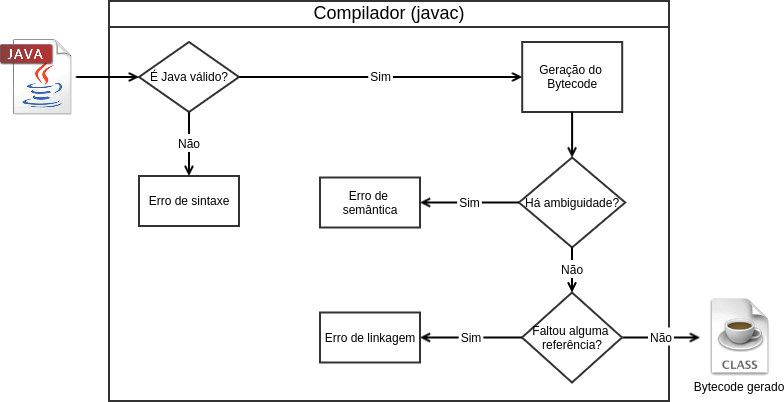
\includegraphics[keepaspectratio,width=1\textwidth,height=1\textheight]{compilation_scheme}
    \end{center}
\end{frame}


\begin{frame}[fragile]{\textit{Bytecode} gerado}
    \begin{minted}{java}
public class Application {
  public Application();
    Code:
       0: aload_0
       1: invokespecial #1 // java/lang/Object."<init>"
       4: return

  public static void main(java.lang.String...);
    Code:
       0: getstatic     #2 // java/lang/System.out
       3: ldc           #3 // Hello, World!
       5: invokevirtual #4 // java/io/PrintStream.println
       8: return
}
    \end{minted}
\end{frame}


\subsection{Execução de uma aplicação}

\begin{frame}{Executando uma aplicação Java}
    \begin{itemize}
        \item[] \icon{eclipse} Eclipse: Pressionar \keys{Ctrl+F11}
            (\menu{\icon{eclipse_run} Run}).

        \item[] \icon{terminal} Terminal: \texttt{java Application}
    \end{itemize}
\end{frame}


\begin{frame}{Execução do \textit{Bytecode} Java}
    \begin{center}
        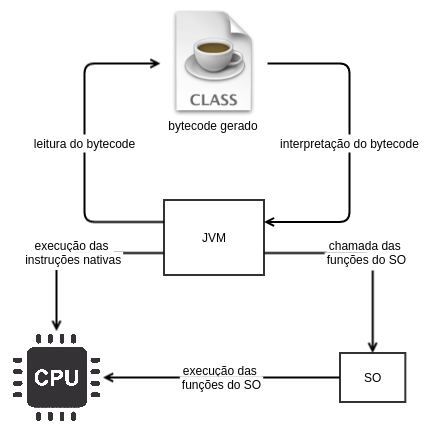
\includegraphics[keepaspectratio,width=1\textwidth,height=0.8\textheight]{jvm_scheme}
    \end{center}
\end{frame}

\begin{frame}[fragile]{Execução do \textit{Bytecode} Java}
    \begin{center}
        \emph{Importante:} A execução do código é sequencial, na ordem em que o
        código foi escrito. Portanto o seguinte de trecho de código:

        \begin{minted}{java}
            System.out.println("Linha 1");
            System.out.println("Linha 2");
            System.out.println("Linha 3");
            System.out.println("Linha 4");
        \end{minted}

        Produzirá a saída:

        \begin{minted}{bash}
            Linha 1
            Linha 2
            Linha 3
            Linha 4
        \end{minted}
    \end{center}
\end{frame}


\section{Trabalhando com programação}

\subsection{Variáveis}
\begin{frame}{Problema: Como guardar valores?}
    Não queremos fazer programas que apenas mostrem textos na tela. Porém, se
    quisermos programas mais complexos, precisamos de mais recursos.
    Para fazer uma loja, por exemplo, precisamos:

    \begin{itemize}
        \item Guardar as informações dos produtos (nomes, preços, etc.);
        \item Guardar a lista de compras do cliente;
        \item Calcular o total da compra para que o cliente possa pagar.
    \end{itemize}
\end{frame}

\begin{frame}{Solução: Variáveis}
    Variáveis são valores guardados na memória (geralmente RAM). Toda variável
    possui:
    \begin{description}
        \item[Identificador:] Nome para referenciá-la no código. Deve ser único
            dentro de um mesmo escopo.
        \item[Tipo:] Define o tipo de dado que ela guarda.
    \end{description}

    Há também, em programação, o conceito de \emph{constantes}, que funcionam
    semelhante às variáveis, porém não podem ser alteradas.
\end{frame}


\begin{frame}[fragile]{Criando uma variável}
    Para criar uma variável, basta \emph{declarar} ela, ou seja, escrever:

    \begin{minted}{java}
        Tipo nome;
    \end{minted}

    É possível ainda criar uma variável e já atribuir um valor a ela, da forma:

    \begin{minted}{java}
        Tipo nome = valor;
    \end{minted}
\end{frame}

\subsection{Tipos de dados}
\begin{frame}{Classificação de tipos}
    Os tipos de dados que podem ser guardados são divididos em:

    \begin{description}
        \item[Tipos Primitivos:] Valores indivisíveis, geralmente números;
        \item[Tipos Definidos por Usuário:] Tipos personalizados, compostos por
            diferentes valores internos.
    \end{description}
\end{frame}

\begin{frame}{Tipos primitivos}
    Numéros inteiros:
    \begin{center}
        \begin{tabular}{|l|l|l|}
            \hline Tipo           & Tamanho & Intervalo \\
            \hline \texttt{byte}  & 1 Byte  & $-128$ a $127$ \\
            \hline \texttt{short} & 2 Bytes & $-2^{15}$ a $2^{15}-1$ \\
            \hline \texttt{int}   & 4 Bytes & $-2^{31}$ a $2^{31}-1$ \\
            \hline \texttt{long}  & 8 Bytes & $-2^{63}$ a $2^{63}-1$ \\
            \hline
        \end{tabular}
    \end{center}

    Numéros reais:
    \begin{center}
        \begin{tabular}{|l|l|l|}
            \hline Tipo            & Tamanho & Intervalo \\
            \hline \texttt{float}  & 4 Bytes & $2^{-149}$ a $(2-2^{-23}) \cdot 2^{127}$ \\
            \hline \texttt{double} & 8 Bytes & $2^{-1074}$ a $(2-2^{-52}) \cdot 2^{1023}$ \\
            \hline
        \end{tabular}
    \end{center}

    Para caracteres há o tipo \texttt{char} (2 Bytes).
\end{frame}

\begin{frame}[fragile]{Operações: Soma}
    \begin{minted}{java}
        int a = 5;
        int b = 7;
        int sum = a + b;
    \end{minted}

    Após executar o trecho acima, o valor de \texttt{sum} será $12$.
\end{frame}

\begin{frame}[fragile]{Operações: Subtração}
    \begin{minted}{java}
        int a = 5;
        int b = 7;
        int diff = a - b;
    \end{minted}

    Após executar o trecho acima, o valor de \texttt{diff} será $-2$.
\end{frame}

\begin{frame}[fragile]{Operações: Multiplicação}
    \begin{minted}{java}
        int a = 5;
        int b = 7;
        int product = a * b;
    \end{minted}

    Após executar o trecho acima, o valor de \texttt{product} será $35$.
\end{frame}

\begin{frame}[fragile]{Operações: Divisão}
    \begin{minted}{java}
        int a = 5;
        int b = 7;
        int quotient = a / b;
    \end{minted}

    Esse é um caso especial em que, após executar o trecho acima, o valor de
    \texttt{quotient} será $0$. Isso se dá porque estamos utilizando números
    \emph{inteiros}.
\end{frame}

\begin{frame}[fragile]{Operações: Divisão real}
    Se quisermos um resultado em números reais, é preciso que \emph{pelo menos
    um dos operandos} seja um número real (\texttt{float} ou \texttt{double}):

    \begin{minted}{java}
        int a = 5;
        double b = 7;
        double quotient = a / b;
    \end{minted}

    (OBS: Se o resultado da divisão for colocada em uma variável que represente
    um inteiro, o resultado será \emph{truncado}, ou seja, o valor após a
    vírgula é ignorado: $1.1 = 1$, $1.9 = 1$).
\end{frame}


\subsection{Declaração de Variáveis}

\begin{frame}{Representando os produtos de uma loja}
    Suponhamos que a tabela de preços da loja seja a seguinte:

    \begin{center}
        \begin{tabular}{|l|l|}
            \hline Produto & Preço \\ \hline
            Pão   & R\$0.50 \\
            Leite & R\$3.00 \\
            Suco  & R\$5.00 \\
            Pizza & R\$9.99 \\
            \hline
        \end{tabular}
    \end{center}

    Assim, precisaremos guardar o preço dos produtos em variáveis.
    Qual o tipo de dado seria mais adequado para representar dinheiro/preço?
\end{frame}

\begin{frame}{Escolhendo o tipo de dado}
    \begin{itemize}
        \item A primeira vista, \texttt{double} e \texttt{float} parecem ótimas
            decições, afinal representam números reais.
        \item \textbf{Porém}, ambos possuem erros de arredondamento, que podem
            fazer ou você ou o cliente perder/ganhar dinheiro por uma simples
            má escolha de tipo de dado.
        \item Por exemplo, às vezes você escreve no código que o valor de um
            \texttt{float} é $4.5$, porém o que efetivamente será carregado é
            $4.4999999999$, que seria o número mais próximo representável por
            um \texttt{float}.
    \end{itemize}
\end{frame}

\begin{frame}{Escolhendo o tipo de dado}
    Para resolver esse problema, algumas linguagens utilizam um tipo de dado
    especial que possui um número fixo de casas decimais, chamado
    \texttt{Decimal} (ou "Fixed Point", em contrapartida com "Floating Point"),
    que pode servir para representar dinheiro (que sempre terá duas casas
    decimais apenas).

    Infelizmente Java não possui esse tipo. Utilizaremos, portanto, o tipo
    \texttt{int}.
\end{frame}

\begin{frame}[fragile]{Declarando as variáveis}
    Assim, a declaração dos preços dos produtos será:

    \begin{minted}{java}
        int breadPrice = 50;
        int milkPrice = 300;
        int juicePrice = 500;
        int pizzaPrice = 999;
    \end{minted}
\end{frame}


\subsection{Interação com o usuário}

\begin{frame}[fragile]{Interagindo com o usuário}
    Em nossa loja será necessário informar a quantidade de cada produto
    que o cliente está levando (para poder calcular o total a ser pago).

    Para isso, é possível pedir ao usuário que digite um texto no Console (ou
    Terminal), ler esse texto e guardar em uma variável:

    \begin{minted}{java}
    System.console().readLine("Digite algo: ");
    \end{minted}
\end{frame}

\begin{frame}[fragile]{Conversão: Texto para número}
    Vale apontar, porém, que o tipo de dado retornado pelo
    \texttt{readLine(\ldots)} é de texto (chamado \textbf{\texttt{String}}). Porém,
    queremos utilizar um tipo numérico, e precisamos converter esse texto para
    um número inteiro. Isso pode ser feito com:

    \begin{minted}{java}
    Integer.parseInt(texto);
    \end{minted}
    E em seguida jogar o resultado em uma variável do tipo inteiro.
\end{frame}

\begin{frame}[fragile]{Interação com o usuário}
    Assim, para pedir ao usuário que digite quantos pães está comprando, basta utilizar:

    \begin{minted}{java}
    String answer = System.console().readLine(
            "Quantidade de pães comprados: "
        );
    int breads = Integer.parseInt(answer);
    \end{minted}

    Ou ainda:

    \begin{minted}{java}
    int breads = Integer.parseInt(
            System.console().readLine(
                "Quantidade de pães comprados: "
            )
        );
    \end{minted}
\end{frame}


\subsection{Estruturas condicionais}

\begin{frame}{Tomada de decisão}
    Em nosso programa, queremos mostrar na tela apenas os produtos que forem
    comprados (afinal, uma loja geralmente tem centenas de produtos
    cadastrados). Porém, como dizer para nosso programa apenas executar um
    trecho de código se e somente se uma condição for satisfeita?

    Ou seja, como podemos fazer nosso programa tomar decisões?
\end{frame}

\begin{frame}[fragile]{Variáveis lógicas}
    Em programação, há um tipo de dado chamado "Lógico", que possui apenas dois
    valores possíveis: \textbf{verdadeiro} e \textbf{falso}. Em Java, esse tipo
    se chama \texttt{boolean}:

    \begin{minted}{java}
    boolean a = true;
    boolean b = false;
    boolean c = 5 > 3; // true
    boolean d = 5 < 3; // false
    \end{minted}
\end{frame}

\begin{frame}{Operadores lógicos}
    \begin{center}
        \begin{tabular}{|c|l|}
            \hline Operador & Descrição \\ \hline
            \texttt{!x} & \texttt{true} se \texttt{x} for \texttt{false} (inversor/NOT). \\
            \texttt{x == y} & \texttt{true} se os valores forem iguais. \\
            \texttt{x $!$= y} & \texttt{true} se os valores forem diferentes. \\
            \texttt{x > y} & \texttt{true} se \texttt{x} for maior do que \texttt{y}. \\
            \texttt{x < y} & \texttt{true} se \texttt{x} for menor do que \texttt{y}. \\
            \texttt{x >= y} & \texttt{true} se \texttt{x} for maior ou igual a \texttt{y}. \\
            \texttt{x <= y} & \texttt{true} se \texttt{x} for menor ou igual a \texttt{y}. \\
            \texttt{x \&\& y} & \texttt{true} se \textbf{ambos} \texttt{x} e \texttt{y} forem \texttt{true} (AND). \\
            \texttt{x || y} & \texttt{true} se pelo menos um dos dois valores forem \\
            & \texttt{true} (OR). \\
            \texttt{x \^{} y} & \texttt{true} se apenas \texttt{x} ou apenas \texttt{y} for \texttt{true}, \\
            & mas \textbf{não ambos ao mesmo tempo}. (XOR). \\
            \hline
        \end{tabular}
    \end{center}
\end{frame}

\begin{frame}[fragile]{Estrutura condicional \texttt{if}}
    Para que nosso programa possa "escolher"\ se vai ou não executar determinado
    trecho, há uma estrutura de código chamada \texttt{if}, em que é entregue
    qualquer valor do tipo \texttt{boolean} entre parênteses e, se durante a
    execução esse valor for \texttt{true}, o trecho de código dentro das chaves
    será executado.

    \begin{minted}{java}
    if (condição) {
        /*
            trecho a ser executado caso a condição
            seja verdadeira
        */
    }
    \end{minted}
\end{frame}

\begin{frame}[fragile]{Exibindo texto no console}
    Assim, para que o produto "Pão"\ seja apenas exibido se for comprado mais
    de um pão, podemos escrever:

    \begin{minted}{java}
    if (breads > 0) {
        System.out.println(
            "Foram comprados " + breads + " pães"
        );
    }
    \end{minted}

    \emph{OBS}: Perceba que é possível juntar textos (\texttt{String}s) com
    outros valores (incluindo outras \texttt{String}s) utilizando "+".
\end{frame}

\begin{frame}{Escolhendo a forma de pagamento}
    Ao final da compra, o cliente irá querer escolher a forma de pagamento.
    Podemos estabelecer três opções:

    \begin{itemize}
        \item Se o usuário digitar "C", o pagamento será efetuado com Cartão;
        \item Se o usuário digitar "D", o pagamento será efetuado em dinheiro.
        \item Para qualquer texto diferente que for digitado o programa irá
            alertar que a opção é inválida.
    \end{itemize}
\end{frame}

\begin{frame}[fragile]{\texttt{If}-\texttt{Else}}
    Para isso, podemos fazer uma opção extra caso um \texttt{if} falhe, através
    de \texttt{else}:

    \begin{minted}{java}
    String paymentForm = System.console().readLine(
        "Escolha a forma de pagamento " +
        "(C = Cartão, D = Dinheiro): "
    );
    if (paymentForm.equals("C")) {
        System.out.println("Escolhido: Cartão.");
    } else if (paymentForm.equals("D") {
        System.out.println("Escolhido: Dinheiro.");
    } else {
        System.out.println("Forma de pagamento inválida.");
    }
    \end{minted}
\end{frame}

\end{document}
